\documentclass[12pt,pdftex,a4paper]{scrartcl}
\usepackage{scrlayer-scrpage}
\usepackage[utf8]{inputenc}
\usepackage[english]{babel}
\usepackage{listings,graphicx,multirow,xcolor}
\usepackage[hyphens]{url}
\usepackage[bf,sf]{caption}
\DeclareCaptionLabelFormat{plain}{\thesection.#2}
\captionsetup[figure]{labelformat=plain,labelsep=quad}

\begin{document}
\title{Automatic role labeling}
	\subtitle{Emotion analysis -- assignment 4}
	\author{Carlotta Quensel\\Felix Bühler\\ Maximilian Wegge}
	\maketitle


\section{Introduction}
As the task of sequence labelling is more advanced than whole-text emotion classification, we expect there to be more difficulties in automatic labelling as well as bigger differences between na\"{i}ve and complex algorithms.

Thus, we decided to do automatic role labeling to confirm these expectations. The sequences for emotion experiencer, target or stimulus are mostly semantically determined and do not directly map onto syntactic structures, but the difference in syntactic structure between different training data might still hold an effect on the results. In this assignment, we look to answer if and how a naive and complex sequence labelling approach differ, as well as compare the influence of different training data on the results. With these objectives as our research questions, we now are able to decide on our method and data.

\section{Method}
Both methods are trained on the same data, so that we can compare the intersection between data and algorithm influences. Therefore, our first step in implementing a role labelling algorithm is to decide on the different data.
\subsection{Training data}
To keep the task mamageable, we only label one role, which is target. The semantic role of emotion target might in a na\"{i}ve understanding correspond to the syntactic role of object (e.g. \textit{I am angry at \textbf{you}.}). This is of course not correct in many instances but still opens an interesting distinction between corpora. As the Reman corpus consists of literary texts, GoodNewsEveryone of news headlines and Electoral tweets of tweets, these three corpora have very different syntactic styles, the news being abbreviated and the literature containing more complex syntactic contructs. While the distribution of our selected role is not ideal between the corpora (Reman only contains around 700 target instances), going forward, these are the three corpora used for training and evaluating both algorithms.

\subsection{Na\"{i}ve approach -- Hidden Markov model}
Sequence labelling in general and the role labelling of emotion target specifically is dependent on the word order, sentence semantic and therefore also syntactical information. While both approaches only consider the tokens as labelling information, while the complex method learns to hopefully detect underlying structures in the token order, the simple method only considers the order of labels. As a basic sequence labelling method, we chose to train a Hidden Markov model and then determine the best label sequence using a viterbi algorithm (the code can be found at the end of this documentation). The model is trained with the token-label pair frequencies relative to the token frequency as emission probabilities and the label bigram frequencies relative to the second token as transition probabilities. An estimated best label sequence therefore combines the most probable label sequence with the highest possibilities of labels for each individual token. The viterbi algorithm is then used to compute this most probable label sequence for a given token sequence. 

While Hidden Markov models have many applications in natural language processing, as a sequence labelling algorithm, it is most frequently used for POS-tagging. In contrast to POS-tagging, a HMM in our case has a deficit, as the tokens are not connected to the tags as strongly. Even though a token can change its syntactical category according to its place in the sentence, there are generally only a few possible labels it can take on. For emotion role labelling on the other hand, a sequence like \textit{my mother} can be the emotion target as well as the experiencer or even the stimulus. The classification mostly depends on semantic information which might be transported through syntactic structure, which our approach does not take into account, as the tokens themselves are only counted as unigrams. Thus, we use a more complex learning approach to combat the problem of missing context. 

\subsection{Complex approach -- Transformer}
For the complex approach, we chose RoBERTa. This deep learning method is an extension of the BERT transformer, which means it is pre-trained on external data. We used 'RoBERTa' to convert the tokenized sentences into an input matrix. This way we can use the whole sequence as context for each individual token. We set a maximum word amount to 100 words, because most of the sequences in our corpora are shorter. The first layer is the pre-trained RoBERTa model\footnote{RoBERTa distribution: \url{https://huggingface.co/transformers/model_doc/roberta.html}}, which was not re-trained, as it has 124 million parameters and therefore superseeds our spacial and temporal constraints. The output is then fed into a bidirectional LSTM with 64 units. Its output is in turn fed into another bidirectional LSTMs of the same make-up. Then we used a Dense-Layer to combine all the features. Thus, the model has the architecture shown in figure \ref{arch}. Adding a residual connection between the first LSTMs and the Dense-Layer improved our accuracy. These layers are used in a Time-Distributed-Layer to produce a prediction for each token. For learning we also added 'ReduceLROnPlateau' to reduce the learning-rate for internal metrics when learning stagnates.

\begin{figure}
\centering 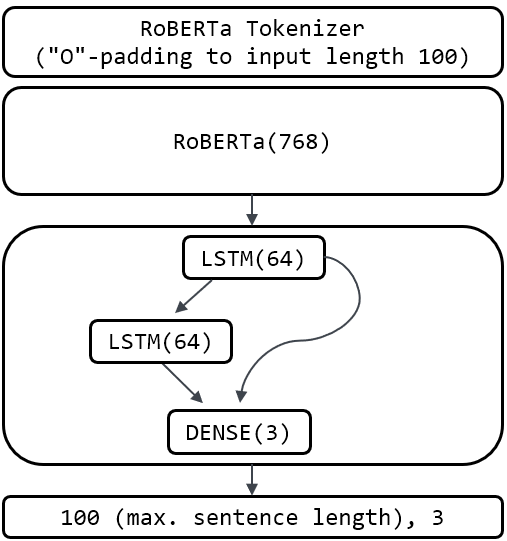
\includegraphics[width=.7\textwidth]{roberta-arch} 

\caption{Model architecture of the RoBERTa with an input layer size of 100 and an output of 3 ('O', 'B' and 'I') for each of the 100 input dimensions.}
\end{figure}

A difficulty with this approach is the sentence length. Since all inputs have the same length, we pad shorter sequences with additional 'O's, thus the model predicts 'outside' at a disproportionate frequency considering the real label counts in the corpora. Reducing the amount of words could improve the predictions, but important information could be cut off (only a problem with the Reman data, as the sentences are very complex and long). Using RoBERTa also influenced the time requirements of our training, e.g. training on "Good News Everyone" took about 3 hours.

\section{Evaluation}
To evaluate our methods, we count intersections between the gold and the predicted 
target sequence as correct labels (True Positives). When a gold label sequence spans more than one predicted sequence or the other way around, we only count one of these multiples and ignore the rest. 

\begin{figure}[h!]
\centering
\begin{tabular}{cc||c|c}
\multicolumn{2}{c||}{} & \multicolumn{2}{c}{\textbf{Gold}}\\
\multicolumn{2}{c||}{} & In & Out\\\hline\hline
\multirow{2}{*}{\rotatebox{90}{\textbf{Pred}}} & In & & \\\cline{2-4}
& Out & &\\
\end{tabular}
\caption{Confusion matrix of the target sequences predicted by the Hidden Markov model trained on the Reman data}
\end{figure}

\appendix
\section{Code}
\subsection{HMM and Viterbi}
\lstinputlisting[language=python]{viterbi.py}

\end{document}
